\documentclass[12pt,onecolumn]{IEEEtran}


\usepackage[utf8]{inputenc}
\usepackage[T1]{fontenc}
\usepackage[spanish,es-tabla]{babel}
\usepackage{amsmath}
\usepackage{graphicx}
\usepackage{hyperref}
\usepackage{cite}
\usepackage{geometry}
\usepackage{float}
\usepackage{booktabs}
\usepackage{array}
\usepackage{siunitx}

\geometry{margin=1in}
\graphicspath{{fig_finales/}}


\title{Proyecto Final: Semáforo Vehicular y Peatonal}

\author{
Gabriel Alonso Chavarría Rodríguez\\
José Andrés Guerrero Araya\\
Julián Murillo Wo Ching\\
Jimena Vargas Vega
}

\date{\today}

\begin{document}

% The paper headers
\markboth{EL3215 Laboratorio de Electrónica Analógica, IS2026}%
{EL3215 Laboratorio de Electrónica Analógica}

\maketitle

\begin{abstract}
En este trabajo se diseñó, simuló y ensambló un circuito eléctrico que replica el funcionamiento de un sistema de semáforos vehicular y peatonal con sistema de audio y cuenta regresiva. Para llevar a cabo este proyecto, se desarrollaron diferentes subsistemas, cada uno encargado de una función específica. El subsistema de alimentación recibe los 120 V AC de un tomacorriente, los rectifica a corriente continua DC y regula el voltaje de 18 V a 5 V. El subsistema contador utiliza el temporizador NE555 para generar una señal de reloj de 1 Hz. El subsistema decodificador toma los pulsos de reloj y los decodifica para los displays que muestran la cuenta regresiva; además, genera las señales necesarias para los cambios de estado. Por su parte, el subsistema controlador realiza los cambios de estado y envía las señales de control para que los demás subsistemas funcionen en el momento adecuado, finalmente, el subsistema de audio se activa cuando el peatón puede cruzar la vía y permanece funcionando durante 20 segundos. En los últimos 5 segundos, el ritmo del sonido aumenta para indicar que el tiempo de cruce está por finalizar.
\end{abstract}

\begin{IEEEkeywords}
Semáforo, FSM, temporización, lógica digital, electrónica analógica.
\end{IEEEkeywords}

%%%%%%%%%%%%%%%%%%%%%%%%%%%%%%%%%%%%%%%%%%%%%%%%%%%%%%%%%%%%%%
\section{Introducción}

Durante el desarrollo de este sistema de semáforo vehicular y peatonal permitió a los estudiantes fortalecer sus habilidades prácticas y conceptuales en electrónica, así como aplicar herramientas como Multisim y EAGLE, técnicas de ensamblado y fabricación de placas de circuito impreso, además la elaboración del proyecto fomentó el trabajo en equipo, la comunicación y la organización para completar el trabajo. 
El proyecto se desarrolló en diferentes etapas, iniciando con el diseño y simulación de los distintos subsistemas, seguido por su implementación física en protoboard y, posteriormente, en circuitos impresos. Durante la etapa de implementación se identificaron diferencias entre el comportamiento obtenido en la simulación y el observado en el circuito real, lo que hizo necesario realizar modificaciones en varios subsistemas para garantizar el cumplimiento de las especificaciones del proyecto dándose los cambios más importantes en la máquina de estados (FSM), el decodificador del sistema de despliegue, la fuente de alimentación y el sistema de audio, mientras que el subsistema de contador mantuvo su diseño original.
La modificación más significativo se dio en el sistema del controlador, que pasó de una lógica con compuertas y flip-flops para los cambios de estado a una lógica basada en un contador CMOS, cuyas salidas se decodifican directamente a los estados del sistema~\cite{harris_digital}, dado esta cambio se tuvo que cambiar otros subsistemas para lograr la compatibilidad con los demás módulos e implementar nuevas soluciones en el sistemas de despliegue y el circuito del botn peatonal. Además se tuvo que incorporar un subsistema de acople adicional para generar la señal $T_C$, diseñada mediante lógica booleana, que indica el instante exacto en que debe ocurrir cada cambio de estado. En el caso de la fuente, se realizaron modificaciones para optimizar el circuito al eliminar resistencias innecesarias, mientras que en el audio se sustituyó la etapa de selección de ritmo originalmente basada en un switch analógico por una lógica combinacional CMOS, por ultimo diversos ajustes derivados de las pruebas experimentales, con el fin de corregir efectos asociados a pérdidas de corriente, caídas de tensión y otras condiciones presentes durante la implementación física.
El informe describe el diseño y funcionamiento de cada uno de los subsistemas que conforman el sistema de semáforo vehicular y peatonal así como la implementación de los circuitos impresos y los resultados obtenidos en el avance final.


%%%%%%%%%%%%%%%%%%%%%%%%%%%%%%%%%%%%%%%%%%%%%%%%%%%%%%%%%%%%%%
\section{Delineamiento del Sistema}

El sistema propuesto se divide en 5 subsistemas básicos: Alimentación, Temporización, Despliegue, Audio, y Máquina de Estados (FSM). Estos subsistemas trabajan entre sí para formar un sistema de dos semáforos peatonales y uno vehicular que funciona para un cruce peatonal. Al apretar alguno de los dos botones adjuntos a los semáforos peatonales, el semáforo vehicular cambia a su luz amarilla. Después de 5 segundos, el vehicular transiciona a luz roja, el peatonal a luz verde, y el sistema empieza a emitir un pitido intermitente de frecuencia constante que indica que el cruce está habilitado para dejar pasar a los peatones. El tiempo que este cruce está habilitado es de 25 segundos. Faltando 5 segundos para finalizar la cuenta regresiva, el tiempo entre pitidos disminuye, indicando que el periodo de cruce está por terminar. Una vez finalizada la cuenta, el sistema vuelve a su estado estándar, con la luz vehicular verde y peatonal roja, hasta que se vuelva a presionar el botón.

El \textbf{subsistema de alimentación} es responsable de proveer el voltaje y corriente que los otros subsistemas necesiten. Tiene el requerimiento de necesitar ser conectado a un tomacorrientes para proveer este poder. Por lo tanto, el subsistema incluye un transformador de voltaje y un circuito rectificador de AC a DC, así como los medios para disipar cualquier potencia restante.

El \textbf{subsistema de temporización} consiste en el reloj que el sistema utiliz para efectuar la cuenta regresiva durante el periodo de paso peatonal. Además, como este subsistema emite un pulso constante cada segundo, brinda una manera de sincronizar señales entre otros subsistemas.

El \textbf{subsistema de despliegue} lidea con llevar el conteo regresivo y desplegarlo en los momentos deseados mediante dos displays de siete segmentos de un dígito. Este subsistema también le entrega a la FSM la información del conteo. De esta manera, la máquina de estados posee la información necesaria para saber en que instantes se debe de cambiar de estado.

El \textbf{subsistema de audio} emite el pitido constante durante el periodo de cruce. Tiene la capacidad de emitir este pitido a dos diferentes frecuencias de ritmo, y así indicar cuando este periodo está por acabar. Se recalca que ninguna de estas dos frecuencias está sincronizada al subsistema de temporización.

\begin{figure}[H]
    \centering
    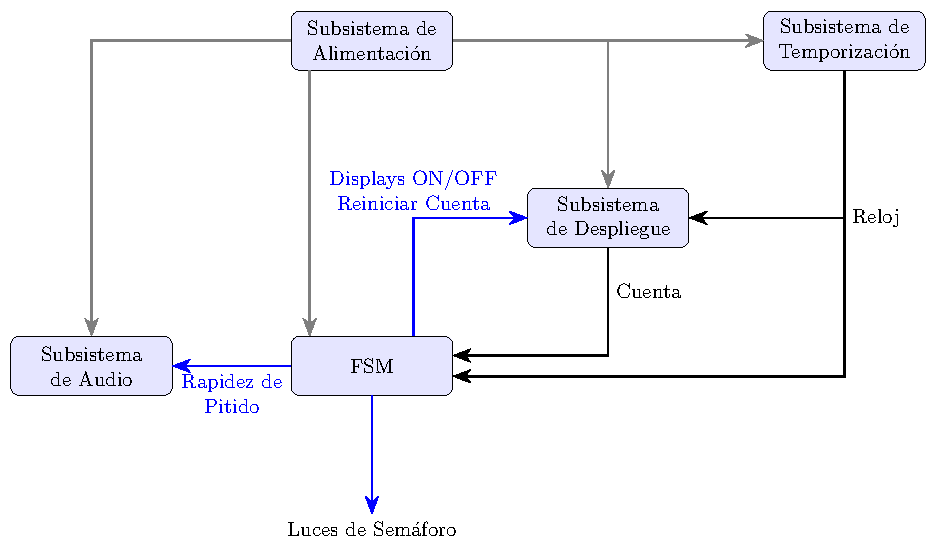
\includegraphics[width=0.9\linewidth]{Diagrama_Bloques_General.pdf}
    \caption{Diagrama de bloques del sistema}
    \label{fig:Diagrama_Bloques_General}
\end{figure}

La \textbf{máquina de estados (FSM)} recibe y emite las señales necesarias para coordinar el funcionamiento completo del sistema. Para llevar esto a cabo, este subsistema se divide en cuatro módulos: contador, botón, señal $T_C$, y los drivers. El contador, similar a los del susistema de despliegue, se utiliza para moverse de manera secuencial entre estados identificables. Cada número en el contador representa un estado diferente. El botón se utiliza para la primera transición de estado, y hacer que el semáforo vehicular pase de una luz roja a amarilla. A partir de este momento, el botón queda deshabilitado, y la máquina de estados le indica al subsistema de despliegue que comience la cuenta regresiva. La señal que indica en qué número se encuentra la cuenta regresiva en cualquier momento dado es recibida por el módulo de la señal $T_C$. Este módulo se encarga de identificar cuando han pasado 5 segundos desde que se inició la cuenta, cuando faltan 5 segundos para finalizar la cuenta, y cuándo se ha finalizado la cuenta. En cada uno de estos instantes, el módulo de la señal $T_C$ le indica al módulo contador que avance al siguiente estado. Una vez que se regresa al estado inicial, el módulo contador rehabilita al botón para poder volver a ser usado.

Finalmente, se tienen los drivers de la FSM. Se tiene un driver por cada estado de la máquina, capaces de entregar una señal en alto proveniente del subsitema de alimentación mientras su respectivo estado sea el actual. A estos drivers están conectadas todas las señales que se desean transmitir desde la máquina de estados. Las más evidentes de estas, son las señales correspondientes a las luces de todos los semáforos. Cada driver está conectado a la configuración de luces que se necesita para su respectivo estado. Sin embargo, también se tienen las señales de cuándo el pitido del subsistema de audio debe habilitarse y aumentar en frecuencia, así como las señales de cuándo se debe comenzar la cuenta regresiva y encender los displays para mostrarla.


\begin{figure}[H]
    \centering
    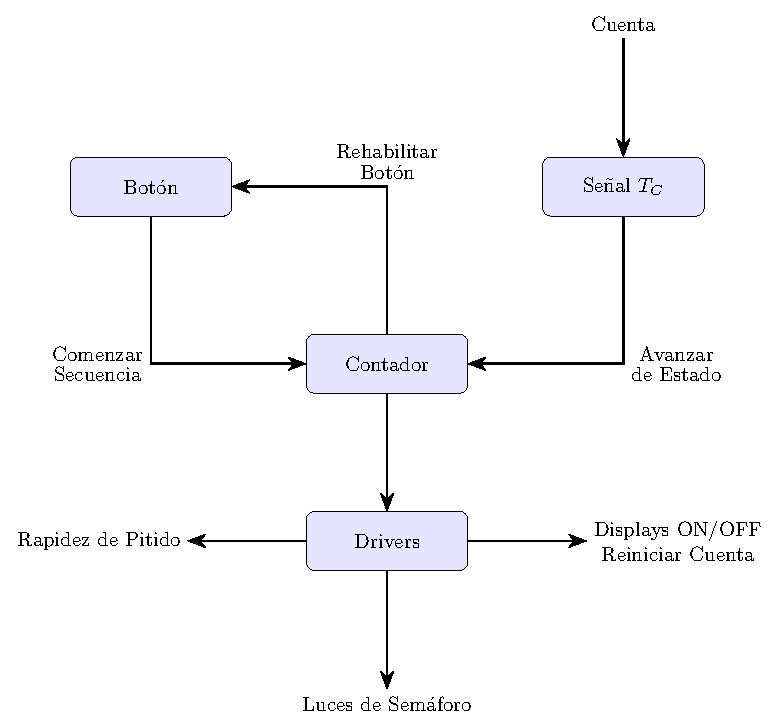
\includegraphics[width=0.9\linewidth]{Diagrama_Bloques_FSM.pdf}
    \caption{Diagrama de bloques de la máquina de estados}
    \label{fig:Diagrama_Bloques_FSM}
\end{figure}

\section{Subsistema de Alimentación}

El voltaje del sistema es proporcionado en su totalidad por una fuente de \qty{120}{VAC}, de manera que el semáforo funciona al ser conectado a un tomacorrientes común. Esta señal pasa por un transformador de \qty{120}{VAC} a \qty{12}{VAC}. La señal de este transformador luego es procesada por un arreglo rectificador de 4 diodos 1N4007 con un capacitor de filtro de \qty{4700}{\mu F}. El subsistema hasta este punto, produce una señal promedio de \qty{15}{V}. Para obtener la señal final en DC, se utilizaron dos reguladores de voltaje LM7805 de \qty{5}{V} en paralelo. Uno de estos reguladores es responsable de la alimentación del subsistema de audio, mientras que el otro actua como fuente para los subsistemas restantes.

\begin{figure}[H]
    \centering
    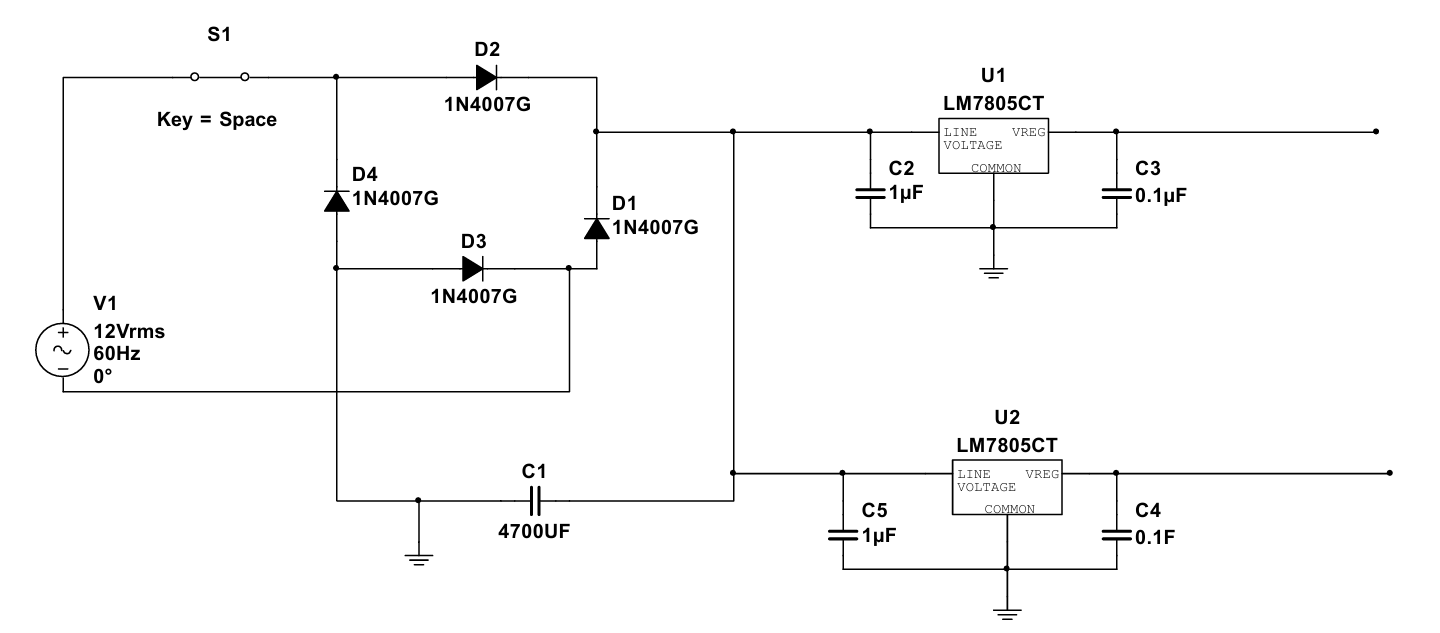
\includegraphics[width=0.9\linewidth]{Diagrama_fuente.png}
    \caption{Subsistema de alimentación rectificador}
    \label{fig:bloque_fuente}
\end{figure}

Además, para ambos reguladores se conectó un capacitor de \qty{1}{\mu F} entre su entrada y tierra. Esto se llevó a cabo para estabilizar el voltaje de entrada que ve el regulador ante ruido que puede aparecer en el circuito rectificador. Además, protege al regulador de caídas en el voltaje de entrada debido a cambios abruptos en la corriente utilizada por el sistema. Asimismo, un capacitor de \qty{0.1}{\mu F} entre su salida y tierra por las mismas razones. \cite{7805datasheet}

La decisión de utilizar dos reguladores en paralelo emergió tras observar muy altas temperaturas en el regulador cuando solo se utilizó uno para la alimentación del sistema completo. El 7805 tiene una corriente máxima de \qty{1.5}{A} \cite{7805datasheet}. Después de una serie de mediciones, se vió que el subsistema de audio requería alrededor de \qty{800}{mA}, mientras que el resto de los subsistemas juntos requeren alrededor de \qty{600}{mA}. Por motivos de seguridad y preservación del sistema, se decidió entonces utilizar un regulador exclusivamente para la alimentación del subsistema de audio, cuya señal fue denotada $V_{CC}$. La señal del regulador responsable por la alimentación del resto de subsistemas se denotó $V_S$.

\section{Subsistema de Temporización}

Para el funcionamiento adecuado del sistema de control, y en general del proyecto, se requiere una señal de reloj que permita establecer una referencia de tiempo para los contadores y la máquina de estados. Por esta razón, se diseñó un circuito basado en el temporizador NE555 en configuración astable, ya que esta configuración permite generar una señal cuadrada periódica sin necesidad de una señal externa de disparo.

La frecuencia de oscilación del 555 en modo astable se aproxima mediante \cite{electronicafp}:

\begin{equation}
	\label{eq:NE555}
    f = \frac{1.44}{(R_A + 2R_B)C}
\end{equation}

El objetivo fue obtener una frecuencia cercana a $1~Hz$, de manera que cada ciclo de la señal represente aproximadamente un segundo dentro del sistema. Inicialmente se seleccionaron valores comerciales para las resistencias y el capacitor, y posteriormente se ajustó el valor de $R_A$ para acercar la frecuencia al valor deseado.

Los valores utilizados fueron:

\begin{itemize}
    \item $R_A = 12~k\Omega$
    \item $R_B = 68~k\Omega$
    \item $C = 10~\mu F$
\end{itemize}

Sustituyendo estos valores en la ecuación:

\begin{equation}
    f = \frac{1.44}{(12k\Omega + 2(68k\Omega))(10\mu F)}
\end{equation}

\begin{equation}
    f \approx 0.973~Hz
\end{equation}

Por lo tanto, el período aproximado es:

\begin{equation}
    T = \frac{1}{f} \approx 1.03~s
\end{equation}

Este valor se considera adecuado para la propuesta de diseño, ya que se encuentra cercano a $1~Hz$ y permite utilizar la salida del 555 como reloj base del sistema. La salida del temporizador se conecta a un LED únicamente como indicador visual durante la simulación (Figura 1).

\begin{figure}[H]
    \centering
    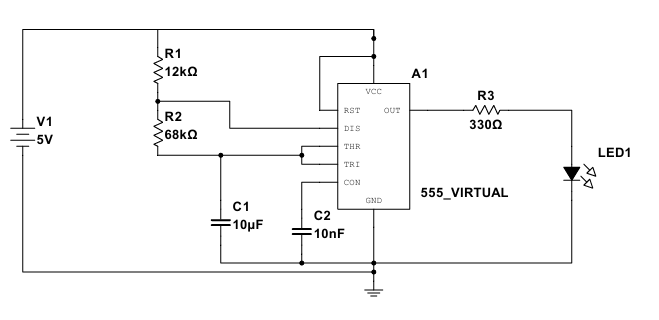
\includegraphics[width=0.9\linewidth]{Diagrama_reloj_555.png}
    \caption{Circuito del reloj de aproximadamente 1 Hz implementado con temporizador 555 en configuración astable.}
    \label{fig:bloque1_555}
\end{figure}

\section{Subsistema de Despliegue}

Este subsistema opera en base a dos contadores CMOS CD4029 conectados en cascodo, uno encargado de contar decenas, y el otro unidades. Ambos contadores se encuentran en modo de contado por década, de modo regresivo, y conectados a la señal de reloj del subsistema de temporización. El contador de decenas se tiene preestablecido empezar en 2, y el de unidades en 5, de modo que se inicie una cuenta regresiva a partir de 25 cuando se habilita el pin de \textit{Preset Enable} de ambos contadores.

Las salidas del contador de las decenas, del bit menos significativo al bit más significativo, se definen $D_0$, $D_1$, $D_2$, y $D_3$. Las salidas del contador de unidades se definen $U_0$, $U_1$, $U_2$, y $U_3$, de la misma manera. Ambos contadores tienen un decodificador CD4511B respectivo, al cuál las salidas del contador están conectadas. Ambos decodificadores están conectados a un display de 7 segmentos de cátodo común correspondiente. El cátodo de estos está conectado a tierra mediante una resistencia de \qty{330}{\Omega} para limitar la corriente. 


\begin{figure}[H]
    \centering
    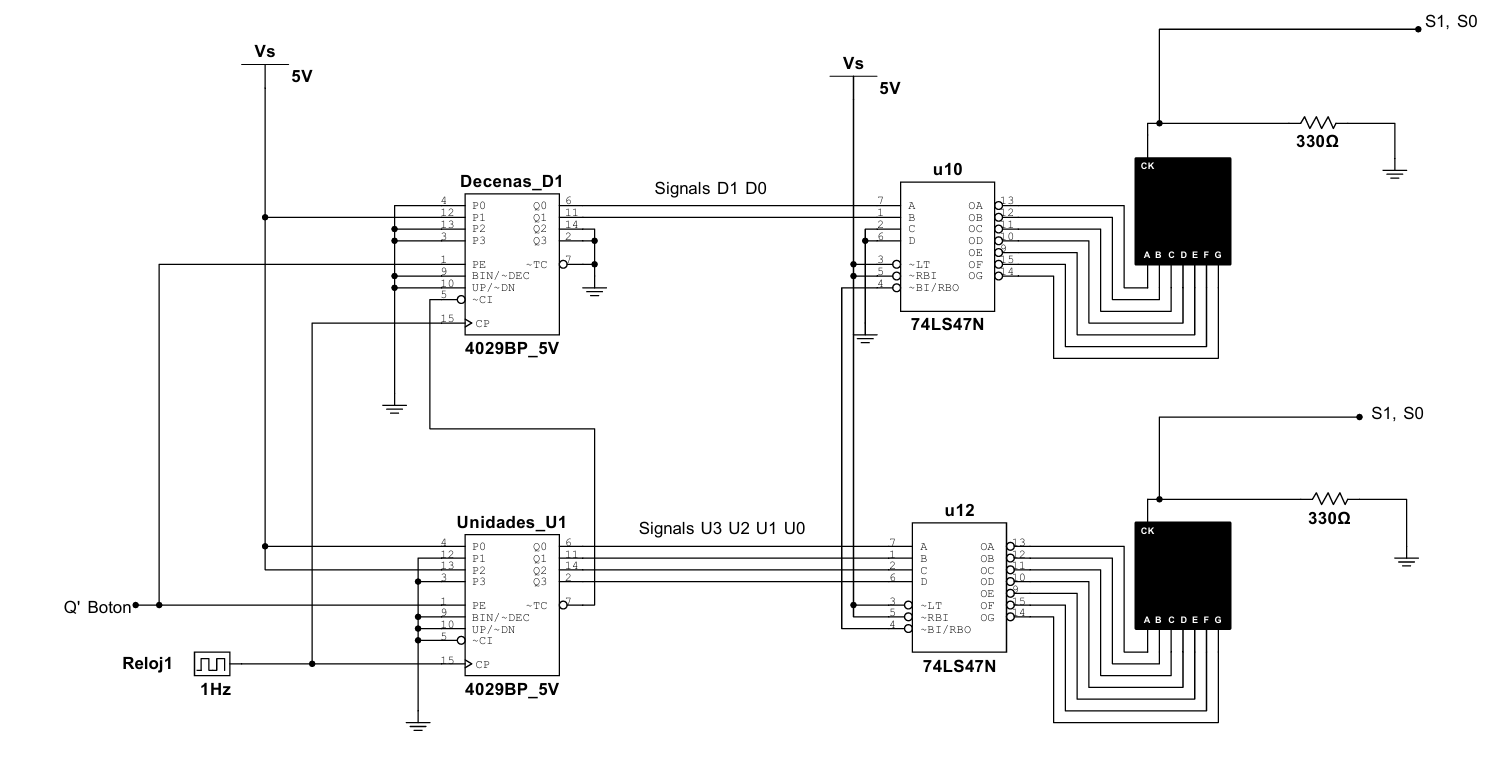
\includegraphics[width=0.9\linewidth]{Diagrama_display.png}
    \caption{Subsistema de decodifiador de los display.}
    \label{fig:bloque_display}
\end{figure}


\section{Subsistema de Audio}

El subsistema de audio tiene como objetivo generar señalización auditiva para el semáforo peatonal. Según las especificaciones del proyecto, el sistema debe producir un sonido periódico mientras el paso peatonal está habilitado, y aumentar la frecuencia de ese sonido durante los últimos cinco segundos antes del cambio al estado de detención.

Para lograr esto se diseñó un subsistema compuesto por tres etapas principales: generación de tono y ritmo mediante temporizadores NE555, selección lógica del ritmo adecuado según la fase del semáforo, y amplificación de la señal para excitar un parlante de $8\,\Omega$.

\subsection{Generación de Tono y Ritmo}

Se utilizaron tres temporizadores NE555 configurados en modo astable~\cite{ne555art}. Esta es la misma configuración que la del 555 en el subsistema de temporización, y permite generar una onda cuadrada de forma autónoma cuya frecuencia depende de los valores de $R_a$, $R_b$ y el capacitor de temporización $C$. Los tres temporizadores cumplen funciones distintas: uno genera el tono audible, uno genera el ritmo lento para el paso peatonal normal, y uno genera el ritmo rápido para los últimos cinco segundos.
\\
\\
\textbf{NE555 de Tono}
Este temporizador genera la frecuencia audible que percibe el peatón. Su salida por el pin~3 produce una onda cuadrada de aproximadamente $300\,\text{Hz}$, representativa de los tonos utilizados en semáforos peatonales reales. Los valores de componentes seleccionados se muestran en la Tabla~\ref{tab:555tono}.

\begin{table}[H]
\centering
\caption{Componentes del NE555 de tono.}
\label{tab:555tono}
\begin{tabular}{lll}
\toprule
\textbf{Componente} & \textbf{Valor} & \textbf{Justificación} \\
\midrule
$R_a$       & $1\,\text{k}\Omega$   & Protege el pin de descarga \\
$R_b$       & $20\,\text{k}\Omega$  & Define la frecuencia junto con $C$ \\
$C$ timing  & $100\,\text{nF}$      & Capacitor de temporización \\
\bottomrule
\end{tabular}
\end{table}

Aplicando la ecuación~\eqref{eq:NE555}:

\begin{equation}
    f = \frac{1{,}44}{(1\,\text{k} + 2\cdot 20\,\text{k})\cdot 100\,\text{nF}}
      = \frac{1{,}44}{41\,000 \times 100\times10^{-9}}
      \approx 351\,\text{Hz}
\end{equation}

El pin~4 (RST) de este temporizador recibe la señal del bloque de selección de ritmo (compuertas AND1A, AND2A, OR1A y AND\_ENABLE1A, ver Subsección~\ref{subsec:seleccion_ritmo}), lo que permite interrumpir el tono rítmicamente para crear los bips audibles.

\begin{figure}[H]
    \centering
    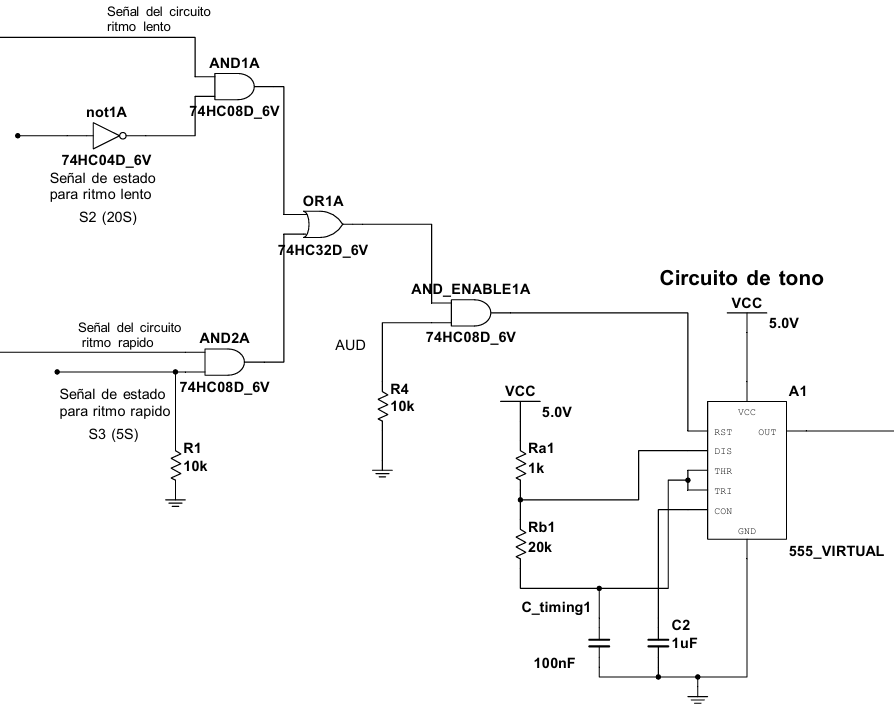
\includegraphics[width=0.9\linewidth]{Diagrama_audio_tono.png}
    \caption{Circuito del NE555 de tono ($\approx 351\,\text{Hz}$).}
    \label{fig:bloque1_555}
\end{figure}

\textbf{NE555 de Ritmo Lento}
Este temporizador genera la cadencia de bips durante la fase normal del paso peatonal. Para lograr una pausa notablemente más larga que el bip, se incorporó un diodo 1N4149 en paralelo con $R_b$, separando los tiempos de carga y descarga del capacitor:

\begin{align}
    t_{\text{HIGH}} &= 0{,}693 \cdot R_a \cdot C \\
    t_{\text{LOW}}  &= 0{,}693 \cdot R_b \cdot C
\end{align}

Los valores seleccionados se muestran en la Tabla~\ref{tab:555lento}.

\begin{table}[H]
\centering
\caption{Componentes del NE555 de ritmo lento.}
\label{tab:555lento}
\begin{tabular}{lll}
\toprule
\textbf{Componente} & \textbf{Valor} & \textbf{Función} \\
\midrule
$R_a$  & $4{,}7\,\text{k}\Omega$ & Duración del bip ($\approx 72\,\text{ms}$) \\
$R_b$  & $6{,}8\,\text{k}\Omega$ & Duración de la pausa ($\approx 104\,\text{ms}$) \\
$C$    & $22\,\mu\text{F}$       & Capacitor de temporización \\
Diodo  & 1N4149                & Separa tiempos de carga y descarga \\
\bottomrule
\end{tabular}
\end{table}

El pin~4 (RST) recibe la señal $AUD$, proveniente de la máquina de estados. Mientras esa señal está en HIGH, el temporizador oscila y genera el ritmo; cuando baja a LOW, el temporizador se detiene y el audio se apaga.

\begin{figure}[H]
    \centering
    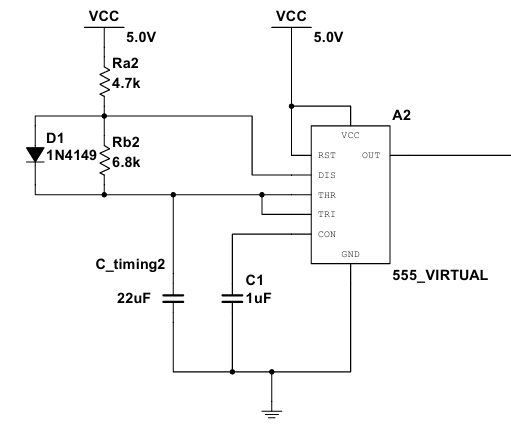
\includegraphics[width=0.7\linewidth]{Diagrama_audio_lento.png}
    \caption{Circuito del NE555 de ritmo lento ($\approx 5{,}7\,\text{Hz}$).}
    \label{fig:ritmo_lento}
\end{figure}

\textbf{NE555 de Ritmo Rápido}
Este temporizador genera la cadencia acelerada durante los últimos cinco segundos del paso peatonal, comunicando urgencia al peatón. Opera con los mismos principios que el de ritmo lento pero con $C$ reducido para aumentar la frecuencia. Los valores se muestran en la Tabla~\ref{tab:555rapido}.

\begin{table}[H]
\centering
\caption{Componentes del NE555 de ritmo rápido.}
\label{tab:555rapido}
\begin{tabular}{lll}
\toprule
\textbf{Componente} & \textbf{Valor} & \textbf{Función} \\
\midrule
$R_a$  & $1\,\text{k}\Omega$    & Duración del bip ($\approx 3\,\text{ms}$) \\
$R_b$  & $20\,\text{k}\Omega$  & Duración de la pausa ($\approx 65\,\text{ms}$) \\
$C$    & $4{,}7\,\mu\text{F}$  & Capacitor de temporización \\
Diodo  & 1N4149                & Separa tiempos de carga y descarga \\
\bottomrule
\end{tabular}
\end{table}

\begin{figure}[H]
    \centering
    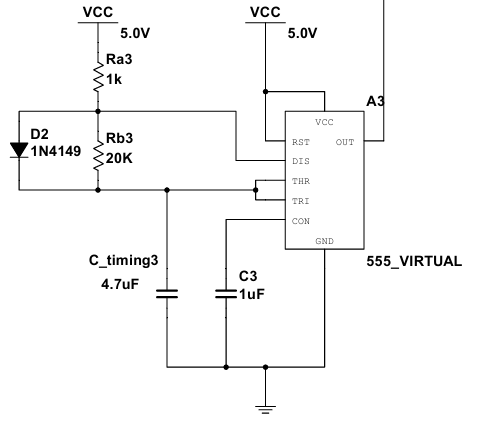
\includegraphics[width=0.7\linewidth]{Diagrama_audio_rapido.png}
    \caption{Circuito del NE555 de ritmo rápido ($\approx 14{,}6\,\text{Hz}$).}
    \label{fig:ritmo_rapido}
\end{figure}

\subsection{Selección Lógica del Ritmo}
\label{subsec:seleccion_ritmo}

Para que el subsistema de audio cambie automáticamente entre ritmo lento y ritmo rápido según la fase del semáforo, se implementó un bloque de selección lógica compuesto por compuertas AND (74HC08), una compuerta OR (74HC32) y un inversor (74HC04), en lugar de un switch analógico.

El inversor (\textit{not1A}) invierte la señal $AF(5S)$ (\textit{últimos 5~s}) proveniente de la máquina de estados. Esta señal, junto con su versión invertida, habilita de forma mutuamente excluyente cuál de las dos señales de ritmo avanza hacia la etapa de tono:

\begin{itemize}
    \item \textbf{AND1A}: combina la salida del NE555 de ritmo lento con $\overline{AF(5S)}$, de modo que solo deja pasar el ritmo lento cuando el sistema \emph{no} se encuentra en los últimos 5~s del cruce peatonal.
    \item \textbf{AND2A}: combina la salida del NE555 de ritmo rápido con $AF(5S)$, de modo que solo deja pasar el ritmo rápido durante los últimos 5~s del cruce peatonal.
\end{itemize}

Ambas señales se combinan mediante la compuerta \textbf{OR1A}, que actúa como un multiplexor de dos entradas cuya señal de control es $AF(5S)$: mientras $AF(5S)$ está en LOW, el ritmo lento pasa a la salida; cuando $AF(5S)$ pasa a HIGH, el ritmo rápido toma el control.

Finalmente, la salida de \textbf{OR1A} se combina con la señal $AUD$ mediante la compuerta \textbf{AND\_ENABLE1A}, que habilita el ritmo seleccionado únicamente durante las fases en que el cruce peatonal está activo ($S_2$ y $S_3$) y lo mantiene en LOW durante el resto del ciclo, evitando que se genere sonido fuera de esos estados. La salida de esta última compuerta alimenta el pin~4 (RST) del NE555 de tono.

\subsection{Etapa de Amplificación}

La señal del pin~3 del NE555 de tono tiene una amplitud de aproximadamente $5\,\text{V}$ con $V_{CC}$~=~\qty{5}{V}, suficiente en voltaje pero con poca capacidad de corriente para excitar directamente un parlante de $8\,\Omega$. Por ello se diseñó un amplificador de dos etapas: emisor común para amplificar el voltaje, seguido de un seguidor de emisor para amplificar la corriente.

Antes de ingresar al amplificador, la señal del NE555 se atenúa mediante un divisor de tensión ($47\,\text{k}\Omega$ en serie, con capacitor de acople de $4{,}7\,\mu\text{F}$) para reducirla de $5\,\text{V}$ a aproximadamente $800$--$900\,\text{mV}$, evitando la saturación del transistor de la primera etapa.

\textbf{Primera etapa: Emisor Común (2N2222).}
La polarización se realiza con un divisor de tensión en la base para establecer el punto Q centrado en $V_{CE} \approx V_{CC}/2$ \cite{2n2222ds}. Los componentes se muestran en la Tabla~\ref{tab:emisor_comun}.

\begin{table}[H]
\centering
\caption{Componentes de la primera etapa (emisor común).}
\label{tab:emisor_comun}
\begin{tabular}{lcc}
\toprule
\textbf{Componente} & \textbf{Valor} & \textbf{Justificación} \\
\midrule
$R_1$ (divisor base, $V_{CC}$) & $47\,\text{k}\Omega$    & Fija la corriente del divisor \\
$R_2$ (divisor base, GND)      & $8{,}2\,\text{k}\Omega$ & Establece $V_B \approx 0{,}74\,\text{V}$ \\
$R_C$ (colector)               & $1{,}2\,\text{k}\Omega$ & Define $I_C$ y el punto Q \\
$C$ acople entre etapas        & $100\,\mu\text{F}$      & Bloquea el DC entre etapas \\
\bottomrule
\end{tabular}
\end{table}

El punto de operación Q se calcula como:

\begin{align}
    V_B &= V_{CC} \cdot \frac{R_2}{R_1 + R_2}
         = 5 \cdot \frac{8{,}2\,\text{k}}{55{,}2\,\text{k}}
         \approx 0{,}74\,\text{V} \\
    I_C &= \frac{V_{CC} - V_{CE}}{R_C}
         = \frac{5 - 2{,}5}{1200}
         \approx 2{,}08\,\text{mA} \\
    V_C &\approx 2{,}9\,\text{V} \quad \text{(medido en simulación)}
\end{align}

\textbf{Segunda etapa: Seguidor de Emisor (TIP31C).}
La configuración de colector común con TIP31C amplifica la corriente para excitar el parlante, presentando alta ganancia de corriente ($h_{FE} \geq 25$ con $I_C = 1\,\text{A}$ según datasheet \cite{tip31ds}) y baja impedancia de salida. Los componentes se listan en la Tabla~\ref{tab:seguidor_emisor}.

\begin{table}[H]
\centering
\caption{Componentes de la segunda etapa (seguidor de emisor).}
\label{tab:seguidor_emisor}
\begin{tabular}{lcc}
\toprule
\textbf{Componente} & \textbf{Valor} & \textbf{Justificación} \\
\midrule
$R_6$ (divisor base, $V_{CC}$) & $820\,\Omega$           & Fija la corriente del divisor \\
$R_7$ (divisor base, GND)      & $2{,}2\,\text{k}\Omega$ & Establece $V_B \approx 2{,}5\,\text{V}$ \\
Parlante (carga)               & $8\,\Omega$             & Carga en el emisor del TIP31C \\
\bottomrule
\end{tabular}
\end{table}

Con $V_B = 2{,}5\,\text{V}$, la corriente y potencia entregadas al parlante resultan:

\begin{align}
    V_E &= V_B - 0{,}7\,\text{V} = 1{,}8\,\text{V} \\
    I_C &= \frac{V_E}{R_L} = \frac{1{,}8}{8} = 225\,\text{mA} \\
    P   &= I_C^2 \cdot R_L = (0{,}225)^2 \times 8 \approx 405\,\text{mW}
\end{align}

Este valor de potencia es suficiente para garantizar la audibilidad del semáforo peatonal en condiciones normales de uso.

\begin{figure}[H]
    \centering
    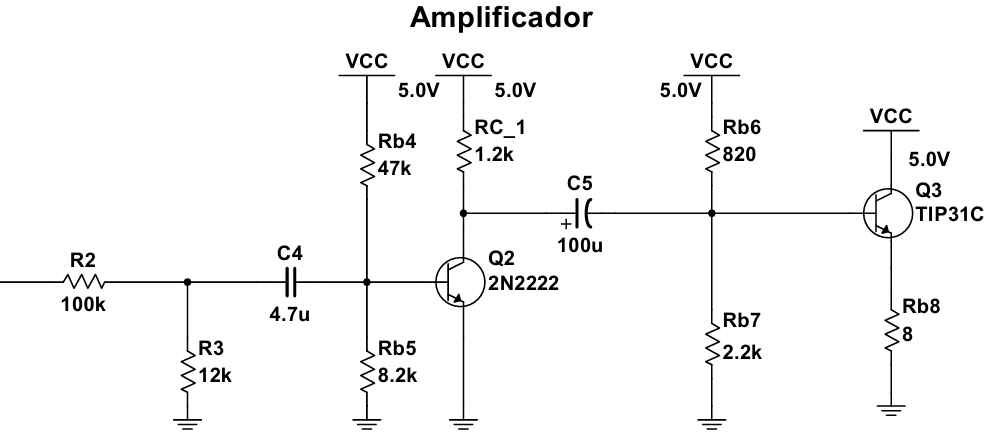
\includegraphics[width=0.9\linewidth]{Diagrama_audio_amplificador.png}
    \caption{Esquemático del amplificador de dos etapas.}
    \label{fig:amplificador}
\end{figure}

\begin{figure}[H]
    \centering
    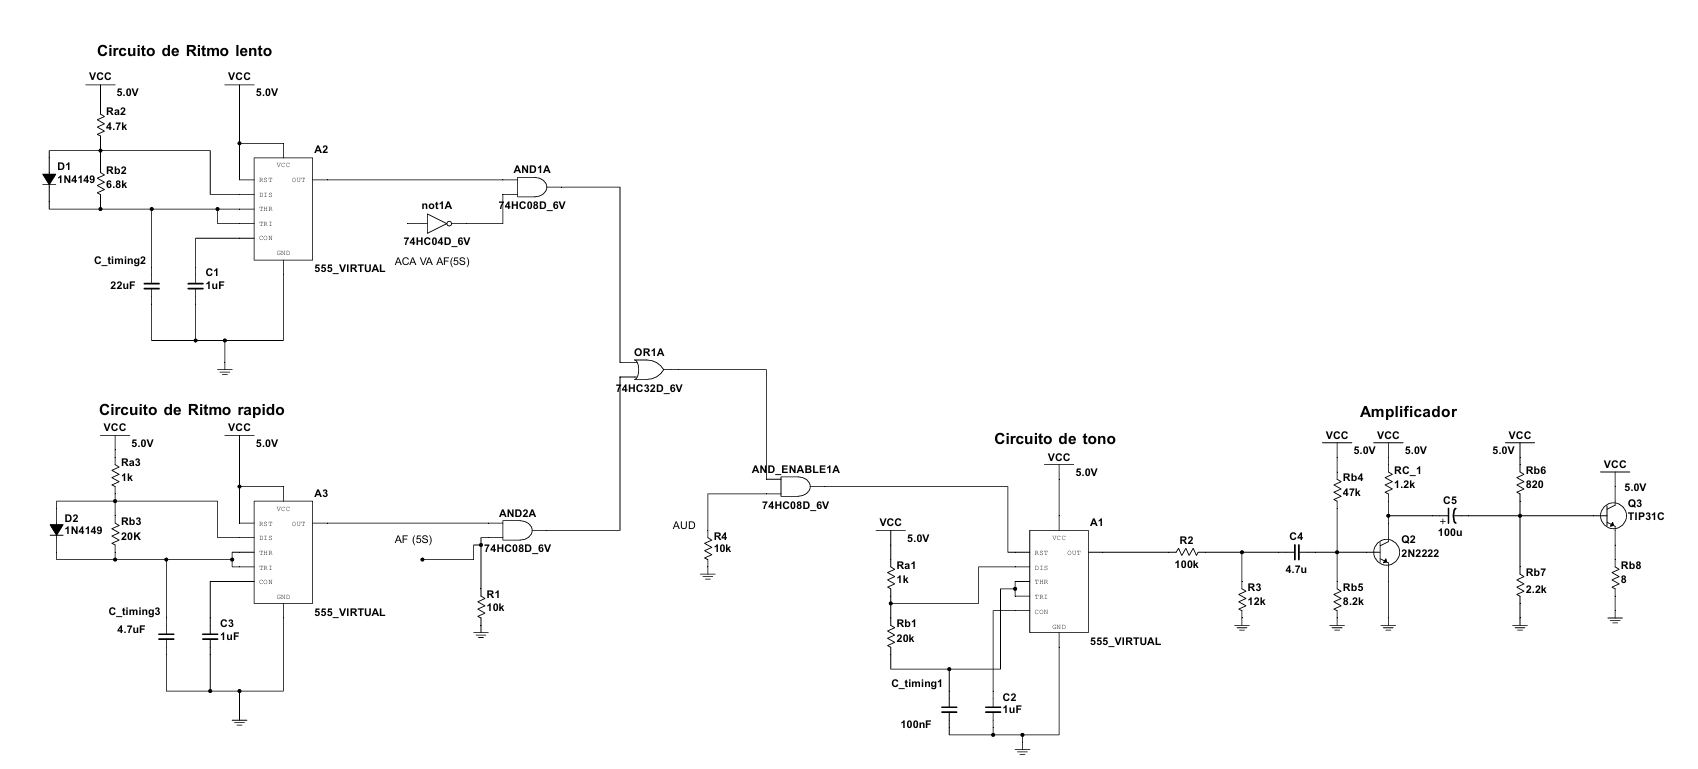
\includegraphics[width=0.9\linewidth]{Diagrama_audio.png}
    \caption{Esquemático completo del subsistema de audio.}
    \label{fig:subsistema_audio}
\end{figure}

%%%%%%%%%%%%%%%%%%%%%%%%%%%%%%%%%%%%%%%%%%%%%%%%%%%%%%%%%%%%%%%%%%%%%%%%%%%%%%%%%%%%%%%%%%%%%%%%%%%%%%%%%%%%%%%%%%%%%%%%%%%%%%%%%%%%%%%%%%%%%%%%%%%%%%%%%%%%%

%% PARTE DE LA FSM

%%%%%%%%%%%%%%%%%%%%%%%%%%%%%%%%%%%%%%%%%%%%%%%%%%%%%%%%%%%%%%%%%%%%%%%%%%%%%%%%%%%%%%%%%%%%%%%%%%%%%%%%%%%%%%%%%%%%%%%%%%%%%%%%%%%%%%%%%%%%%%%%%%%%%%%%%%%%%%%%%%%%%%%%%%%%%%%

\section{Máquina de estados (FSM)}

En la Figura~\ref{fig:maquina_estados} se presenta el diagrama de la máquina de estados con el comportamiento del semáforo, mostrando las cuatro combinaciones de LEDs vehiculares y peatonales, la señal de audio activa en cada caso, la duración de los estados temporizados, y las condiciones de transición ($T_B$ y $T_C$) entre ellos y los detalles de implementación de cada uno de estos elementos se desarrollan en las subsecciones siguientes.

\begin{figure}[H]
    \centering
    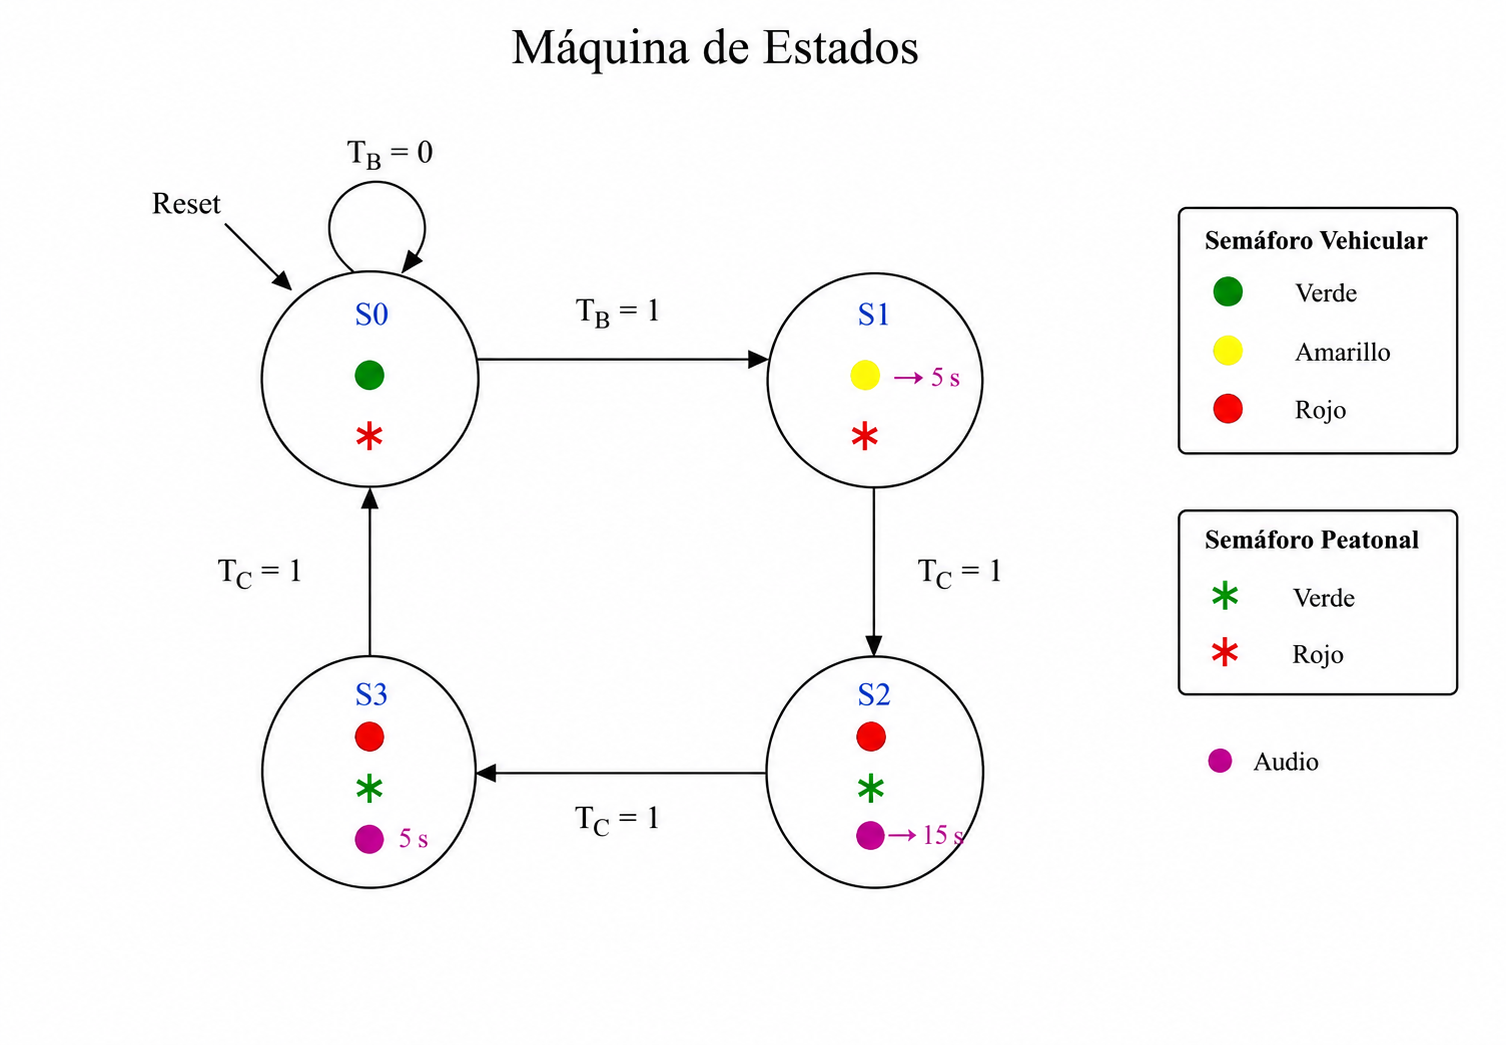
\includegraphics[width=0.7\linewidth]{fsm.png}
    \caption{Diagrama de la máquina de estados finitos del semáforo.}
    \label{fig:maquina_estados}
\end{figure}

\subsection{Estados} %Describir a qué está conectado el driver de cada estado (LEDs, cátodo, señal de audio, etc)

En esta sección se quiere mencionar cómo las señales tomadas de los 4 drivers interactúan con el resto del sistema. De esta manera, se puede tener el panorama completo de cómo funciona el sistema en su totalidad durante cada estado. 

\begin{table}[H]
\centering
\caption{Resumen de LEDs y audio activos por driver}
\label{tab:estados_resumen}
\begin{tabular}{ccccc}
\toprule
\textbf{Driver} & \textbf{Vehicular} & \textbf{Peatonal} & \textbf{Audio} & \textbf{Duración} \\
\midrule
Driver 0 ($S_0$) & Verde & Rojo & --- & Indefinida \\
Driver 1 ($S_1$) & Amarillo & Rojo & --- & 5~s \\
Driver 2 ($S_2$) & Rojo & Verde & Ritmo lento & 15~s \\
Driver 3 ($S_3$) & Rojo & Verde & Ritmo rápido & 5~s \\
\bottomrule
\end{tabular}
\end{table}

Cabe destacar que, físicamente, el semáforo peatonal cuenta con cuatro LEDs (dos por cada extremo de la calle: rojo y verde), pero ambos pares se controlan con la misma pareja de señales lógicas provenientes de la FSM, de modo que los LEDs de ambos lados de la calle conmutan siempre de forma idéntica.

\subsubsection{S0}

Es el estado inicial del sistema, correspondiente al Driver~0. En este estado se enciende el LED verde del semáforo vehicular, permitiendo el paso de vehículos, y el LED rojo del semáforo peatonal, indicando que el cruce no está habilitado. Ninguna señal de audio está activa. El sistema permanece en $S_0$ por tiempo indefinido hasta que el botón peatonal es presionado, momento en el cual se libera el \textit{Preset Enable} de la FSM y se habilita la cuenta regresiva de 25~s del subsistema de despliegue.

\subsubsection{S1}

Corresponde al Driver~1. El semáforo vehicular cambia a amarillo, advirtiendo a los conductores del cambio inminente a rojo, mientras que el semáforo peatonal se mantiene en rojo. Ninguna señal de audio está activa. Este estado dura 5~s, al cabo de los cuales $T_C = 1$ lleva a la FSM al Driver~2 ($S_2$).

\subsubsection{S2}

Corresponde al Driver~2. El semáforo vehicular cambia a rojo y el semáforo peatonal cambia a verde, habilitando el cruce. Se activa la señal $AUD$, que habilita el temporizador NE555 de ritmo lento ($\approx 5{,}7\,\text{Hz}$), produciendo la cadencia de bips normal del cruce peatonal. Este estado dura 15~s, al cabo de los cuales $T_C = 1$ lleva a la FSM al Driver~3 ($S_3$).

\subsubsection{S3}

Corresponde al Driver~3. Los LEDs vehicular (rojo) y peatonal (verde) se mantienen iguales que en $S_2$, por lo que visualmente no hay cambio en el semáforo. Lo que cambia es la señalización auditiva: la señal $AF(5S)$ (\textit{últimos 5~s}) conmuta el bloque de selección lógica (Subsección~\ref{subsec:seleccion_ritmo}) para que el NE555 de ritmo rápido ($\approx 14{,}6\,\text{Hz}$) tome el control del tono, advirtiendo al peatón que el tiempo de cruce está por terminar. Transcurridos estos 5~s (25~s totales desde que se presionó el botón), $T_C = 1$ avanza la cuenta de la FSM a 4, condición equivalente al Driver~0 ($S_0$), lo cual además dispara el \textit{Clear} del botón y reinicia el ciclo completo.

\subsection{Contador y Drivers}

La máquina de estados está basada en un contador CMOS CD4029 sincronizado al reloj del sistema. Este se utilizó por su capacidad de poder moverse entre diferentes estados de manera secuencial y reinicio asincrónico. Se utilizaron sus dos primeras salidas $Q_0$ y $Q_1$, correspondientes a los dos bits menos significativos de la cuenta, para representar los cuatro estados necesarios. En conjunto a una compuera AND CD4081 y una NOT CD4069 se pasó de esta cuenta en binario de dos bits a una condificación \textit{one-hot}, donde se tiene solo una señal en alto por cada uno de los diferentes estados. Cada una de de estas señales se usó como señal de activación para su propio driver, cuyo esquemático se puede ver en la Figura \ref{fig:driver_esquematico}. El resultado es una FSM que se mueve de manera secuencial entre cuatro estados cuándo esta recibe una señal de conteo síncrona con el reloj del sistema. Cada estado tiene su respectivo driver, el cuál permite accessar la alimentación de \qty{5}{V} solamente cuando su respectivo estado está activo.

Se definen los cuatro estados, junto a sus respectivas señales de driver, como $S0$, $S1$, $S2$, y $S3$. Las cuatro señales de salida del contador de la FSM, del bit menos significativo al bit más significativo, como $Q_0$, $Q_1$, $Q_2$, y $Q_3$. 

\begin{figure}[H]
    \centering
    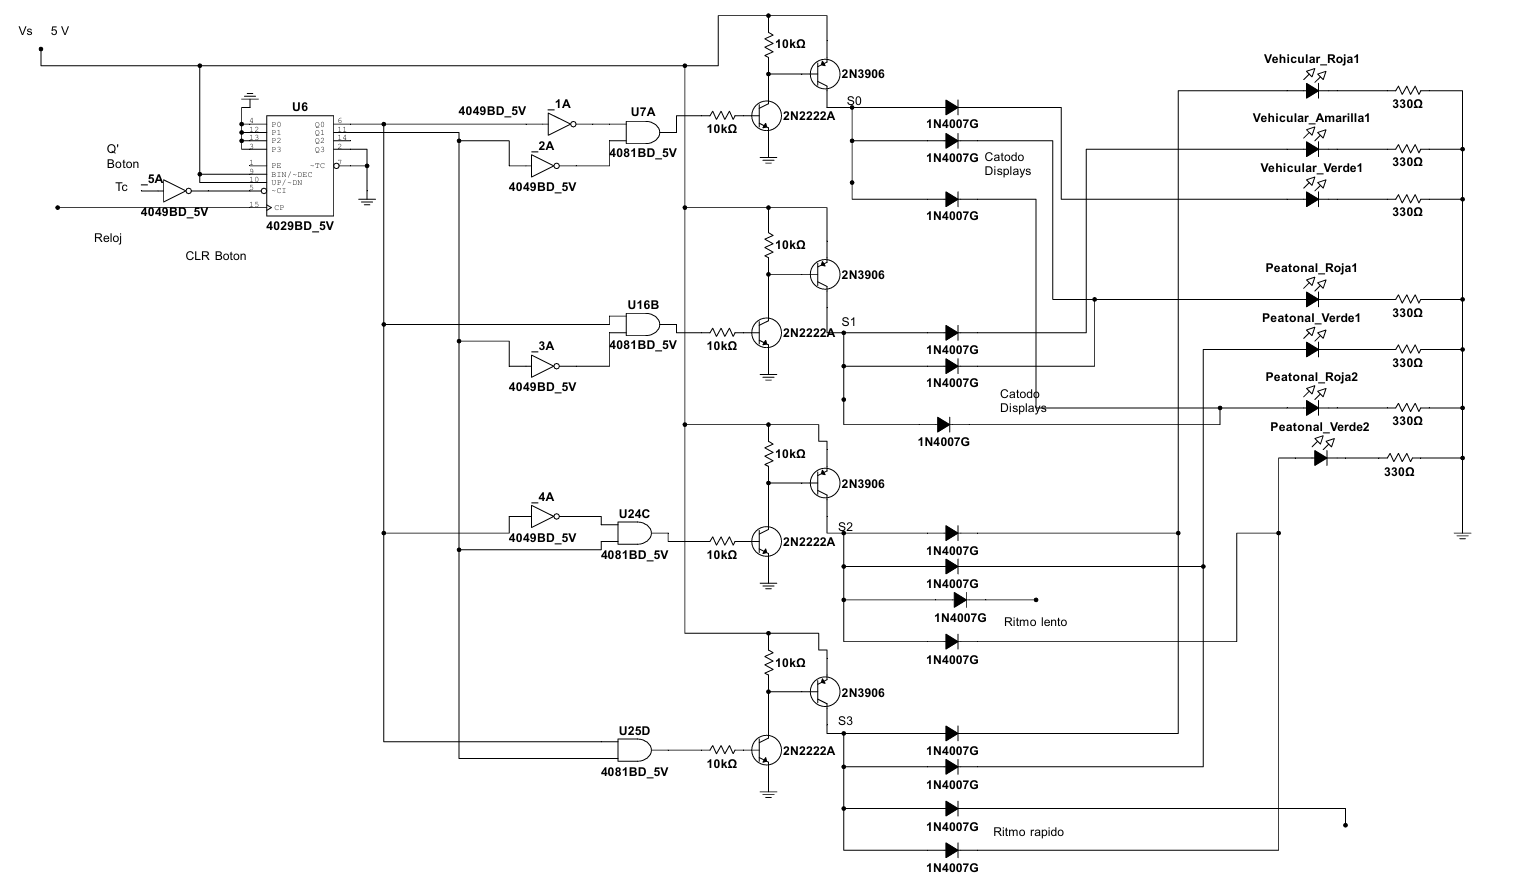
\includegraphics[width=0.9\linewidth]{Diagrama_fsm.png}
    \caption{Esquemático de drivers en FSM}
    \label{fig:driver_esquematico}
\end{figure}


\begin{table}[H]
\centering
\caption{Desglose de codificación one-hot}
\label{tab:Drivers/Estados}
\begin{tabular}{cccccc}
\toprule
\textbf{Estado} & \textbf{Bits de Contador} & \textbf{Cuenta en FSM} & \textbf{Driver Activo} \\
\midrule
$S0$ & $\overline{Q_2}~\overline{Q_1}~ \overline{Q_0}$ & 0 & Driver 0 \\
$S1$ & $\overline{Q_2}~\overline{Q_1} ~Q_0$ & 1 & Driver 1 \\
$S2$ & $\overline{Q_2}~Q_1 ~\overline{Q_0}$ & 2 & Driver 2 \\
$S3$ & $\overline{Q_2}~Q_1 ~Q_0$ & 3 & Driver 3 \\
$S0$ & $Q_2~\overline{Q_1}~ \overline{Q_0}$ & 4 & Driver 0 \\
\bottomrule
\end{tabular}
\end{table}


El número preestablecido del contador se configuro para ser 0, de manera que todas sus salidas se niegan una vez que el pin de \textit{Preset Enable} recibe una señal en alto. En el sistema, \textit{Preset Enable} recibe la señal de salida del botón $\overline{Q}$, por lo que el contador de la FSM se encuentra perpetuamente en el estado $S0$ hasta que el botón sea activado. Una vez que el el botón se activa, su señal $\overline{Q}$ permanecerá baja, lu cuál le permitirá a la FSM cambiar a estados diferentes de $S0$.


La transición de un estado a otro es controlada por la señal $T_C$. Está sera explicada a fondo más adelante. Se recalca que el conteo del CD4029 se habilita mediante el pin de \textit{Carry-In}, el cuál está negado. Por lo tanto, la señal $T_C$ que recibe esta entrada usualmente se encuentra en alto, y se pone baja de manera síncrona durante un pulso del reloj cuendo se quiere que la FSM avance al siguiente estado. 

\subsection{Botón}

Como se mencionó anteriormente, el bóton cumple la función de controlar cuándo el contador de la FSM, así como los contadores en el subsistema de despliegue, se encuentran en su modo preestablecido. El diseño del botón está basado en el flip-flop SN7474, en conjunto con un buffer inversor SN7404. El uso de un flip-flop es crucial para poder guardar la "decisión" de apretar el botón hasta que la FSM regrese a su estado inicial. De esta manera, volver a apretar el botón durante un estado no deseado no tiene efecto alguno.


Dado que, al encender el sistema por primera vez, el 7474 tiene la posibilidad de comenzar en cualquiera de sus dos estados, se tuvo que divisar una manera de que el pin de \textit{Clear} siempre reciba una señal baja en este momento. Para esto se utilizó otro de los inversores del 7404. Se conectó la entrada de un inversor a $V_S$ mediante un capacitor de \qty{10}{\mu F}, así como a tierra mediante una resistencia de \qty{10}{k\Omega}. La salida de este inversor se conectó al pin de \textit{Clear}.

Cuándo el circuito se enciende, este capacitor se encuentra descargado, por lo que actúa brevemente como un corto entre $V_S$ y la entrada del inversor. Esto permite que \textit{Clear} reciba una señal baja cuando el switch del subsistema de alimentación es cerrado. Posteriormente a este evento, el capacitor se logra cargar a los \qty{5}{V} de $V_S$, actuando como un abierto hasta que el sistema sea apagado. Una vez que este capacitor se carga, la entrada del inversor es fijada en bajo mediante la resistencia de \qty{10}{k\Omega}, lo cuál le envía perpetuamente una señal en alto al pin de \textit{Clear} y permite el funcionamiento ordinario del sistema. 

\begin{figure}[H]
    \centering
    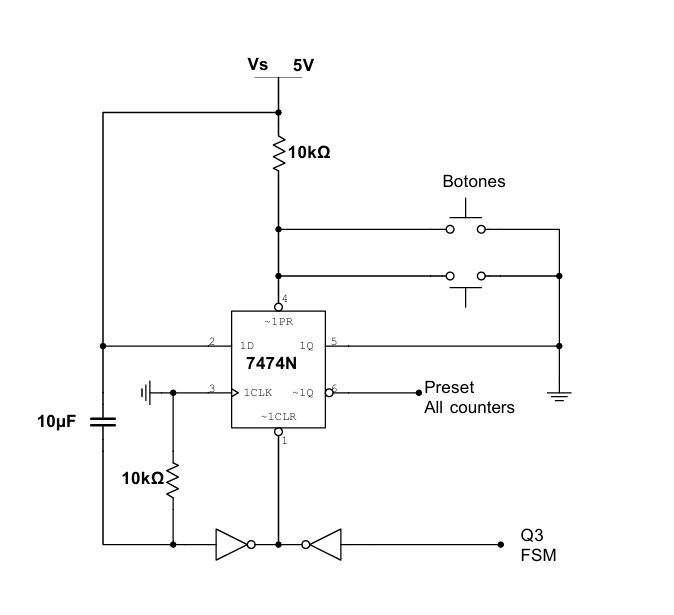
\includegraphics[width=0.6\linewidth]{Diagrama_boton.png}
    \caption{Esquemático del circuito del botón peatonal.}
    \label{fig:diagrama_boton}
\end{figure}





\subsection{Señal $T_C$}

La señal $T_C$ es generada por lógica combinacional a partir de las salidas de los contadores de decenas ($D_0$--$D_3$) y unidades ($U_0$--$U_3$) del subsistema de despliegue, mediante la red de compuertas 4049, 4002, 4081 y 4072 que decodifican los valores específicos de la cuenta regresiva de 25~s en los que debe ocurrir una transición de estado.

Esta señal ingresa al pin \textit{Carry-In} (negado) del contador CD4029 de la FSM, habilitando un incremento de su cuenta interna cada vez que se activa. $T_C$ permanece normalmente en alto (conteo deshabilitado) y se pone en bajo de forma síncrona con el reloj del sistema en los siguientes instantes de la cuenta regresiva:

\begin{itemize}
    \item \textbf{Cuenta de despliegue = 20} (5~s después del botón): $T_C = 1 \Rightarrow$ la cuenta de la FSM avanza de 1 a 2 ($S_1 \to S_2$).
    \item \textbf{Cuenta de despliegue = 5} (20~s después del botón): $T_C = 1 \Rightarrow$ la cuenta de la FSM avanza de 2 a 3 ($S_2 \to S_3$).
    \item \textbf{Cuenta de despliegue = 0} (25~s después del botón): $T_C = 1 \Rightarrow$ la cuenta de la FSM avanza de 3 a 4, condición equivalente a $S_0$ (ver Tabla~\ref{tab:Drivers/Estados}). Este último pulso, a través de $\overline{Q_2}$, dispara además el pin \textit{Clear} del botón descrito anteriormente, reiniciando el ciclo completo.
\end{itemize}

La transición inicial de la cuenta 0 ($S_0$) a la cuenta 1 ($S_1$) no depende de $T_C$, sino de la liberación del pin de \textit{Preset Enable} de la FSM al presionar el botón peatonal, la cual permite que su contador comience a incrementar con el siguiente pulso de reloj disponible.

De esta manera, la duración efectiva de cada estado queda determinada por el intervalo entre disparos consecutivos de $T_C$: 5~s para $S_1$, 15~s para $S_2$, y 5~s para $S_3$, sumando los 25~s totales de la cuenta regresiva del subsistema de despliegue.

\begin{figure}[H]
    \centering
    \includegraphics[width=0.9\linewidth]{Diagrama_tc.png}
    \caption{Lógica combinacional de generación de la señal $T_C$ a partir de las salidas de los contadores de decenas y unidades.}
    \label{fig:diagrama_tc}
\end{figure}

\section{Diseño e implementación del PCB de alimentación}

Como parte de la implementación final del proyecto, se diseñó y fabricó una PCB correspondiente al subsistema de alimentación. Esta etapa permitió trasladar el circuito de la protoboard a una placa física más compacta, reduciendo la cantidad de conexiones externas y facilitando su integración con la maqueta del semáforo vehicular y peatonal.

El diseño del PCB se realizó en EAGLE, tomando como base el esquemático del subsistema de alimentación (Fig~\ref{fig:diagrama_pcb_eagle}). En la placa se incluyeron los diodos rectificadores 1N4004, el capacitor principal de filtrado de \qty{4700}{\mu F}, los dos reguladores 7805, capacitores de desacople en la entrada y salida de los reguladores, y borneras para la conexión de entrada y salidas de alimentación. Los reguladores se colocaron en encapsulado vertical con disipadores de calor, debido a la corriente requerida por los demás subsistemas y a la disipación térmica observada durante las pruebas.

Para el diseño físico, la placa se diseñó de una sola cara, por lo que las pistas fueron trazadas en la capa \textit{Bottom}, mientras que los componentes se insertaron desde la capa \textit{Top}. Además, se incorporó un plano de tierra conectado a GND, cubriendo la mayor área posible del PCB. Este plano permite mantener una referencia común de tierra y facilita el proceso de fabricación, ya que reduce la cantidad de cobre que debe ser removido.

Entre el plano de tierra y las pistas se dejó una región de aislamiento para evitar cortocircuitos. En el diseño se utilizó un aislamiento mayor al mínimo recomendado, debido a las limitaciones de la broca utilizada durante el proceso de fabricación. De esta manera, se buscó asegurar que la máquina pudiera remover correctamente el cobre entre pistas, pads y plano de tierra. Asimismo, se utilizaron pistas de mayor grosor en las líneas de alimentación, ya que estas transportan la corriente requerida por los distintos bloques del sistema.

Antes de fabricar la placa, se verificó el diseño mediante la herramienta DRC de EAGLE, revisando separaciones, pads, ancho de pistas y continuidad de las conexiones. A su vez se aplicaron las correcciones y consejos dados por el profesor. Posteriormente, se procedió con la fabricación del PCB, el perforado de los pads y el proceso de soldadura de los componentes. Finalmente, se realizaron pruebas de continuidad y medición de voltaje en las salidas de los reguladores para comprobar el funcionamiento correcto del subsistema de alimentación.  En la Fig.~\ref{fig:pcb_bottom} se puede observar una acumulación de estaño alrededor del pad de GND correspondiente al capacitor C1. Este inconveniente ocurrió durante el proceso de soldadura y fue corregido parcialmente retirando el exceso de material, se verificó que no existieran cortocircuitos con pistas cercanas antes de continuar con las pruebas de funcionamiento del PCB.

En las Figuras~\ref{fig:diagrama_pcb_eagle}, \ref{fig:pcb_eagle}, \ref{fig:pcb_antes}, \ref{fig:pcb_top} y \ref{fig:pcb_bottom} se muestra el proceso de implementación del PCB, desde el diseño en EAGLE hasta la placa fabricada y ensamblada.

\begin{figure}[H]
    \centering
    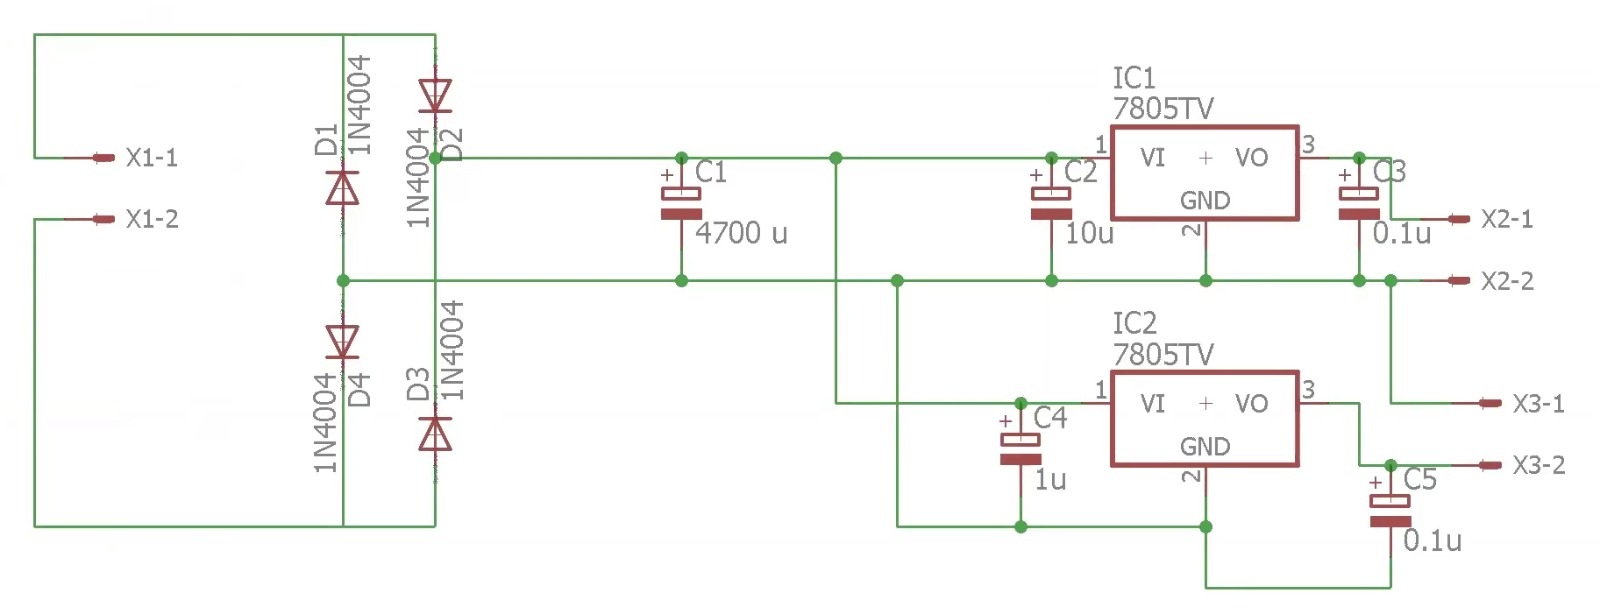
\includegraphics[width=0.9\linewidth]{Diagrama_pcb.png}
    \caption{Esquemático del diseño del PCB del subsistema de alimentación en EAGLE.}
    \label{fig:diagrama_pcb_eagle}
\end{figure}

\begin{figure}[H]
    \centering
    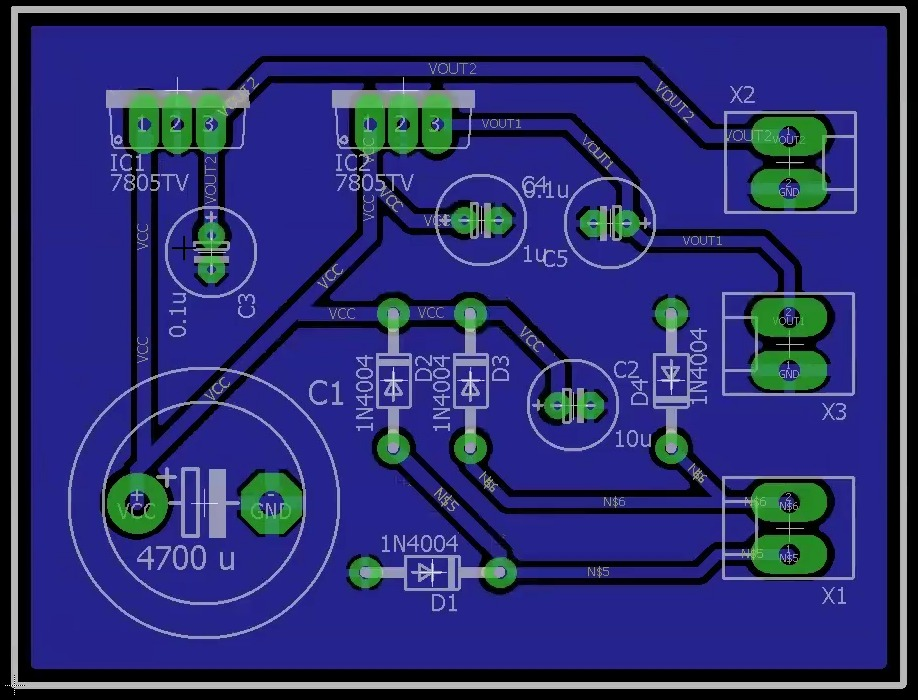
\includegraphics[width=0.9\linewidth]{pcb_eagle.png}
    \caption{Diseño del PCB del subsistema de alimentación en EAGLE.}
    \label{fig:pcb_eagle}
\end{figure}

\begin{figure}[H]
    \centering
    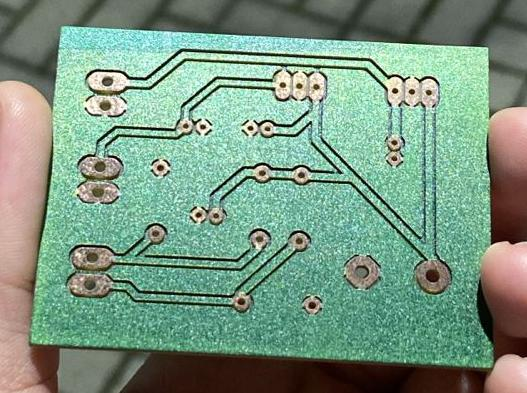
\includegraphics[width=0.85\linewidth]{pcb_antes.jpg}
    \caption{PCB fabricado antes del proceso de soldadura.}
    \label{fig:pcb_antes}
\end{figure}

\begin{figure}[H]
    \centering
    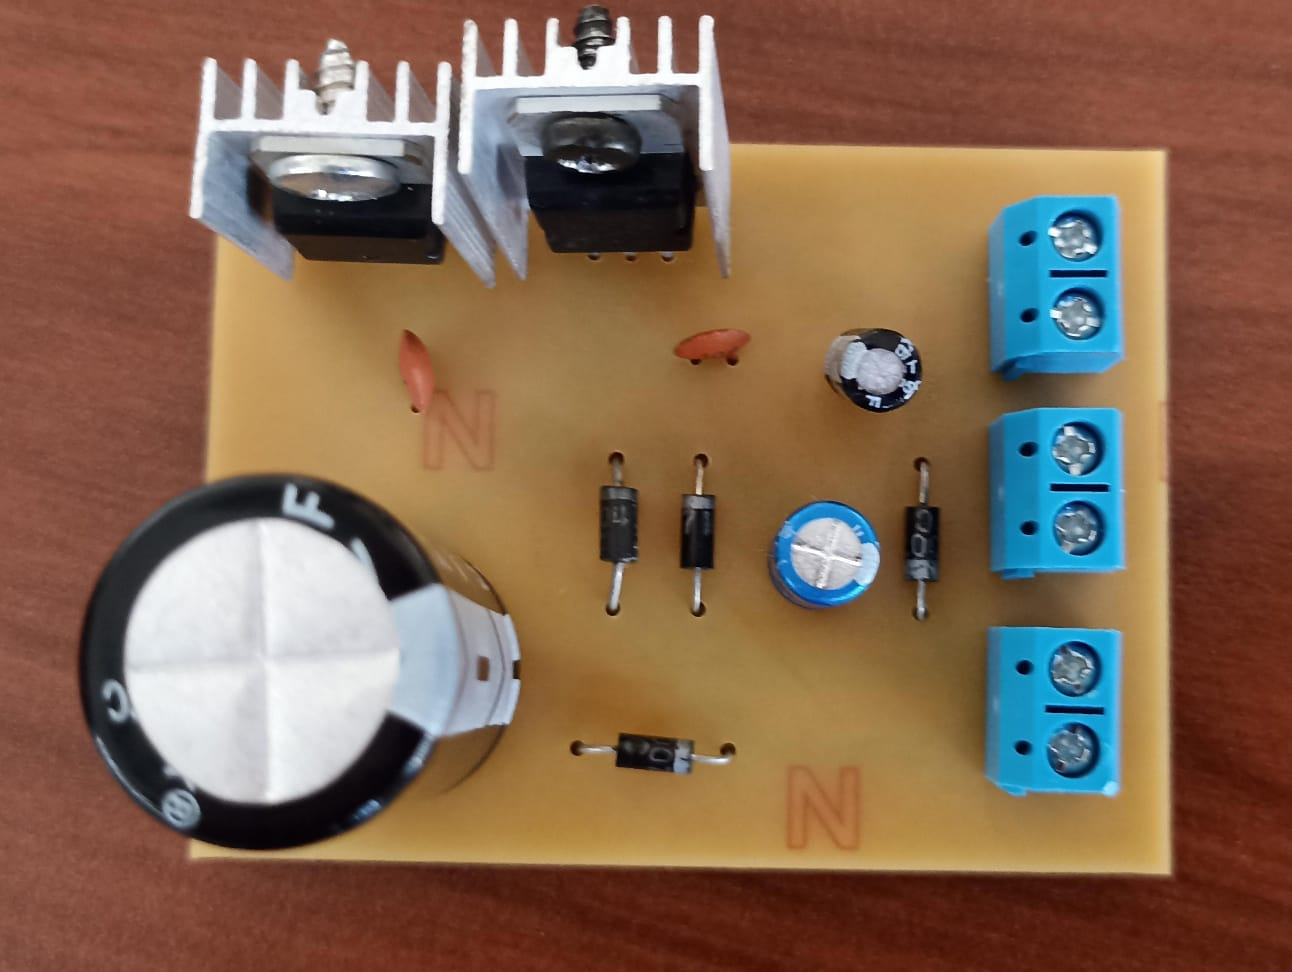
\includegraphics[width=0.85\linewidth]{pcb_despues1.jpg}
    \caption{PCB del subsistema de alimentación con los componentes soldados, visto desde la capa superior.}
    \label{fig:pcb_top}
\end{figure}

\begin{figure}[H]
    \centering
    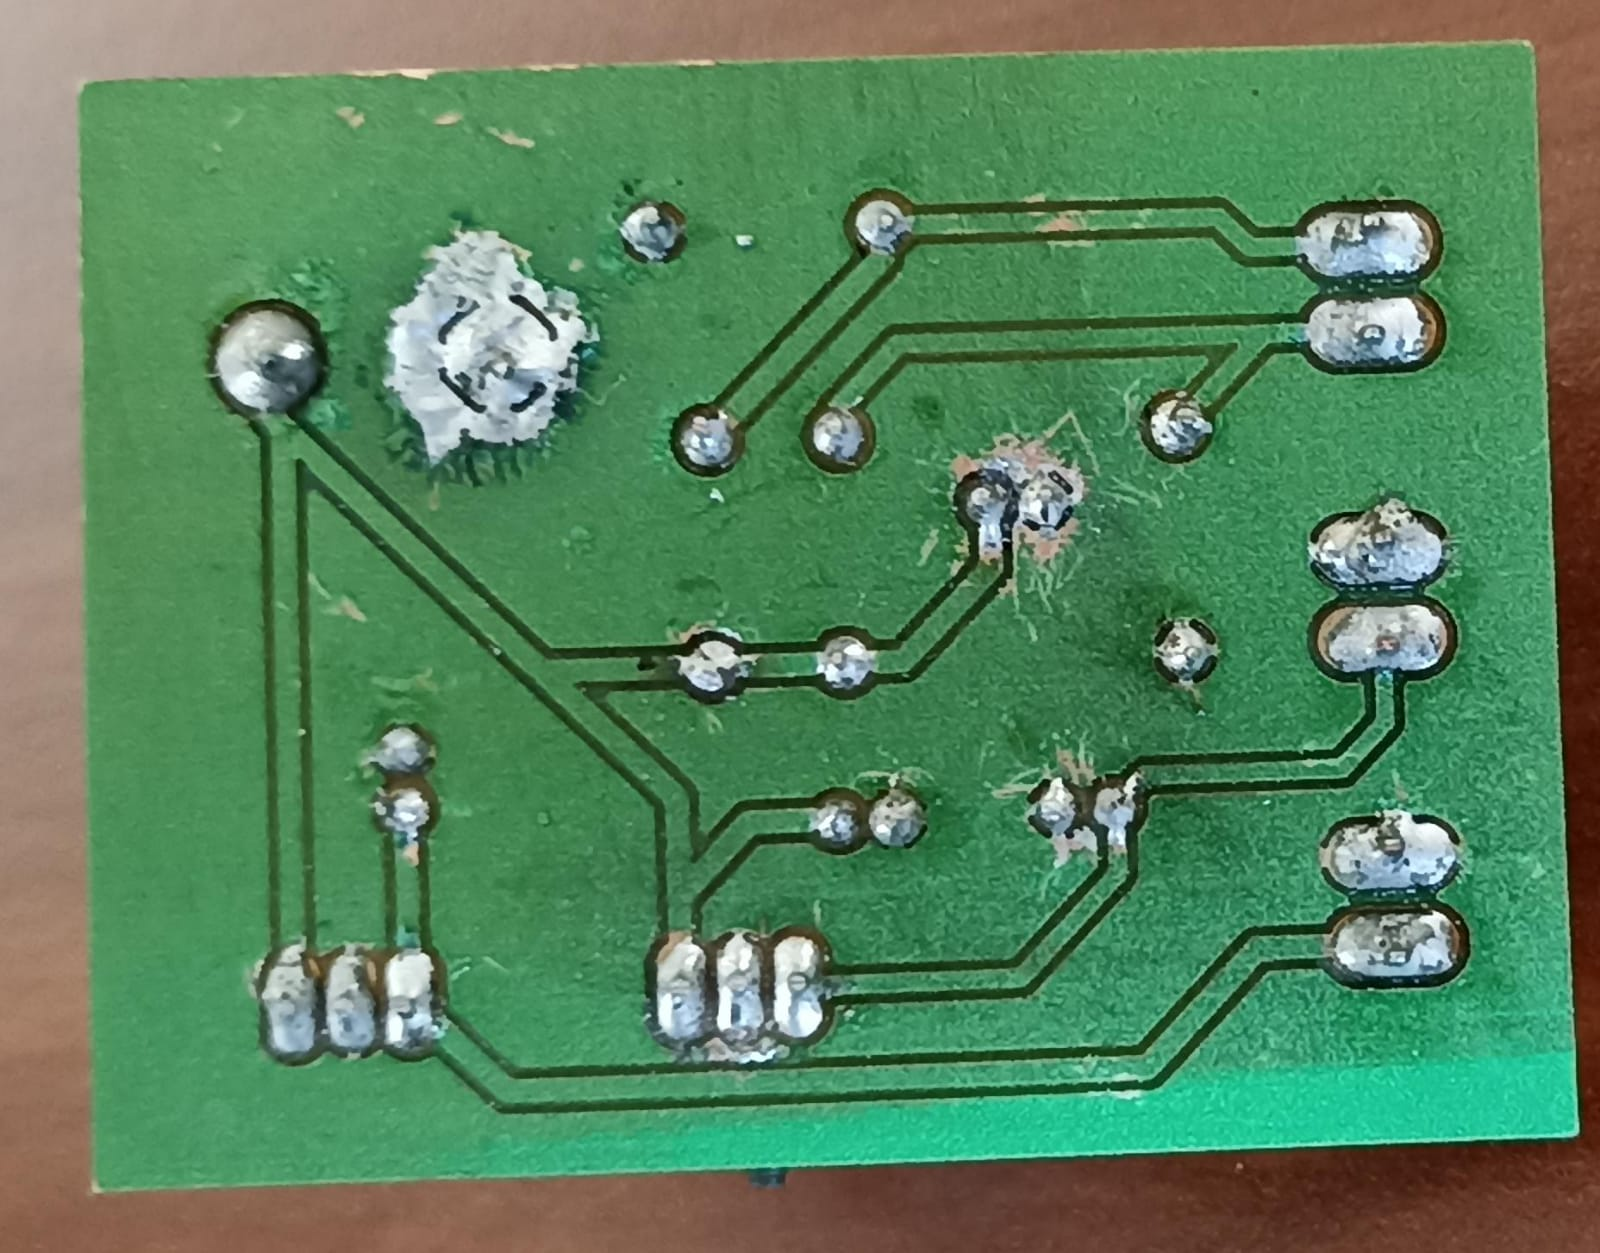
\includegraphics[width=0.85\linewidth]{pcb_despues2.jpg}
    \caption{Vista inferior del PCB después del proceso de soldadura.}
    \label{fig:pcb_bottom}
\end{figure}


\section{Maqueta}

Para el diseño de la maqueta se buscó representar un cruce peatonal realista, relacionado con el entorno que transitan los integrantes del curso por lo que la intersección que inspiró el diseño fue la ubicada frente a la entrada principal del Instituto Tecnológico de Costa Rica, el objetivo era utilizar un entorno familiar tanto para el profesor como para los estudiantes; sin embargo, dado que en la realidad esa intersección no cuenta con semáforo vehicular ni peatonal, el diseño se adaptó para emplearla como referencia visual del proyecto.


Para su construcción se utilizaron los siguientes materiales:

\begin{itemize}
    \item Papel de construcción
    \item Cartón de presentación
    \item Pajillas
    \item Hojas blancas
    \item Pinturas
    \item Pegamento
    \item Silicón
\end{itemize}

\begin{figure}[H]
    \centering
    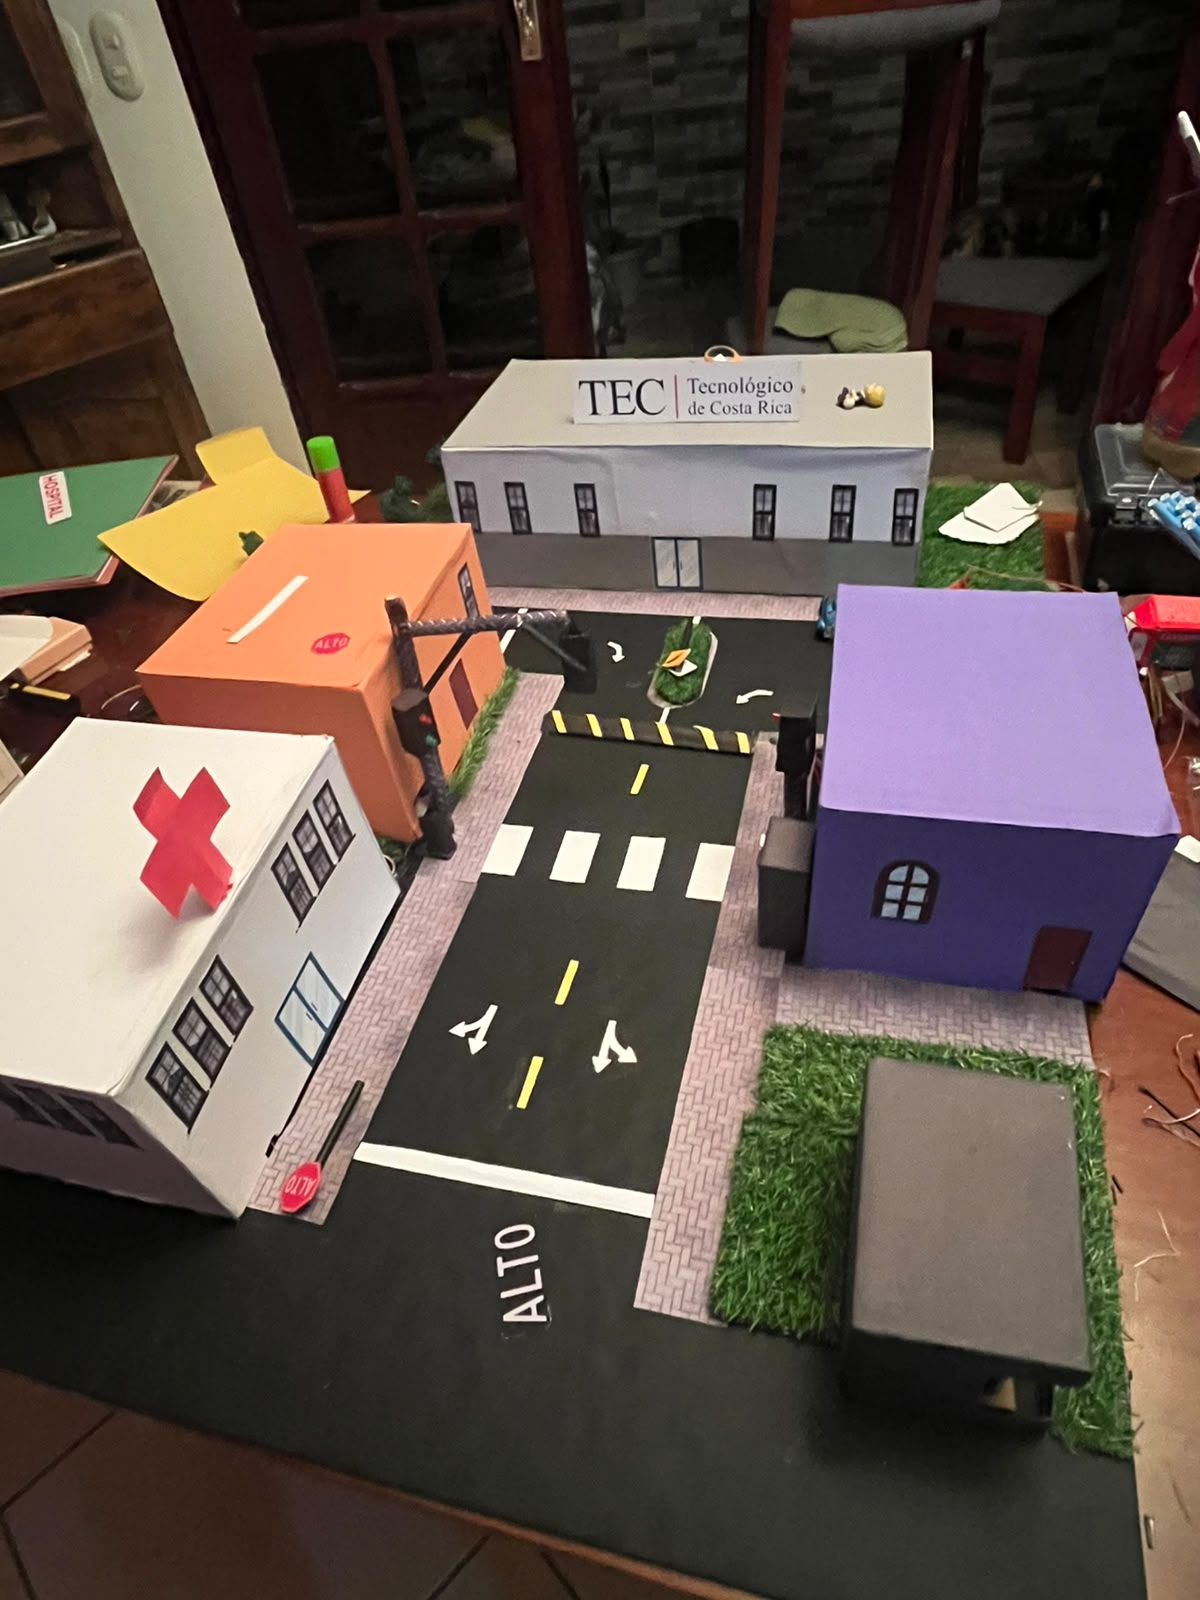
\includegraphics[width=0.7\linewidth]{maqueta.jpeg}
    \caption{Diseño final de la maqueta.}
    \label{fig:maqueta}
\end{figure}

%%%%%%%%%%%%%%%%%%%%%%%%%%%%%%%%%%%%%%%%%%%%%%%%%%%%%%%%%%%%%%
\begin{thebibliography}{99}
\bibitem{74ls74datasheet}
Texas Instruments, ``SN74LS74A Dual D-Type Positive-Edge-Triggered Flip-Flops With Preset and Clear Datasheet,'' Dallas, TX, USA. [Online]. Available: \url{https://c1555f5ec9.clvaw-cdnwnd.com/34662fcf1f1e607c561442431023ac8e/200000751-dcad7dda84/74LS74%20Datasheet.pdf}

\bibitem{7805datasheet}
onsemi, MC7800, MC7800A, MC7800AE, NCV7800 Positive 1.0 A Voltage Regulators Datasheet, Rev. 28, Apr. 2014. [Online]. Available: https://www.onsemi.com/pdf/datasheet/mc7800-d.pdf



\bibitem{electronicafp}
Electrónica FP, ``555 Astable,'' YouTube, 2021. [Online]. Available: \url{https://www.youtube.com/watch?v=OKDaA-yE2QY}
\bibitem{2n2222ds}
Philips Semiconductors, ``2N2222 NPN Switching Transistors,'' datasheet, Philips Semiconductors, Eindhoven, Netherlands. [Online]. Available: \url{https://www.alldatasheet.com/html-pdf/15067/PHILIPS/2N2222/995/4/2N2222.html}. [Accessed: May 2026].

\bibitem{tip31ds}
ON Semiconductor, ``TIP31, TIP31A, TIP31B, TIP31C: NPN Epitaxial Silicon Transistor,'' datasheet, ON Semiconductor, Phoenix, AZ, USA. [Online]. Available: \url{https://www.alldatasheet.com/html-pdf/499213/ONSEMI/TIP31/214/1/TIP31.html}. [Accessed: May 2026].

\bibitem{ne555art}
Ariat Tech, ``What is the NE555?'' \textit{Ariat Tech Blog}, 2024. [Online]. Available: \url{https://www.ariat-tech.es/blog/what-is-the-ne555.html#t2}. [Accessed: May 2026].


\bibitem{harris_digital}
D. M. Harris and S. L. Harris, \textit{Digital Design and Computer
Architecture}, 2nd ed. Morgan Kaufmann, 2013.


\end{thebibliography}

\end{document}
